\documentclass[11pt]{beamer}
\usepackage[utf8]{inputenc}
\usepackage[T1]{fontenc}
\usepackage{lmodern}
\usepackage{amsmath}
\usepackage{amsfonts}
\usepackage{amssymb}
\usepackage{graphicx}
\usetheme{cambridgeUS}
\usepackage[longnamesfirst]{natbib} 
\usepackage{caption}
\DeclareCaptionFormat{citation}{%
	\ifx\captioncitation\relax\relax\else
	\captioncitation\par
	\fi
	#1#2#3\par}
\newcommand*\setcaptioncitation[1]{\def\captioncitation{\textit{Source:}~#1}}
\let\captioncitation\relax
\captionsetup{format=citation,justification=centering}
\usepackage {subcaption}
\usepackage{CJKutf8}
%代码设置
\usepackage{verbatim}
\usepackage{cprotect}
\usepackage{listings}
\usepackage{color}
\usepackage{xcolor}
\usepackage{showexpl} 
\lstloadlanguages{[LaTeX]Tex} 
\lstset{ %
	language=TeX,                % the language of the code
	basicstyle=\footnotesize,           % the size of the fonts that are used for the code
	numbers=left,                   % where to put the line-numbers
	numberstyle=\tiny\color{black},  % the style that is used for the line-numbers
	stepnumber=1,                   % the step between two line-numbers. If it's 1, each line 
	% will be numbered
	%numbersep=5pt,                  % how far the line-numbers are from the code
	backgroundcolor=\color[RGB]{254,249,231},      % choose the background color. You must add \usepackage{color}
	showspaces=false,               % show spaces adding particular underscores
	showstringspaces=false,         % underline spaces within strings
	showtabs=false,                 % show tabs within strings adding particular underscores
	frame=single,                   % adds a frame around the code
	frameround=tttt
	rulecolor=\color{black},        % if not set, the frame-color may be changed on line-breaks within not-black text (e.g. commens (green here))
	tabsize=2,                      % sets default tabsize to 0 spaces
	captionpos=b,                   % sets the caption-position to bottom
	breaklines=true,                % sets automatic line breaking
	breakatwhitespace=false,        % sets if automatic breaks should only happen at whitespace
	title=\lstname,                 % show the filename of files included with \lstinputlisting;
	% also try caption instead of title
	keywordstyle=\color{blue},          % keyword style
	commentstyle=\color[RGB]{17,122,101},       % comment style
	%	stringstyle=\color{mauve},         % string literal style
	escapeinside={\%*}{*)},            % if you want to add LaTeX within your code
	morekeywords={*,...}               % if you want to add more keywords to the set
}

\definecolor{myred}{RGB}{231, 76, 60}

\begin{document}
	
	\begin{CJK*}{UTF8}{gkai}
		
	\author[LC Meng]{Lingchao Meng}
	\title[LaTeX Tutorial]{\LaTeX\ Tutorial}
	%\subtitle{}
	%\logo{}
	\institute[SE, PKU]{School of Economics\\Peking University}
	%\date{}
	%\subject{}
	%\setbeamercovered{transparent}
	%\setbeamertemplate{navigation symbols}{}
\begin{frame}[plain]
    \maketitle
\end{frame}

\begin{frame}
	This is  just a beginners guide to writing documents in \LaTeX\ without prior knowledge of \LaTeX. This slide is designed for the \LaTeX\ workshop at School of Economics, Peking University.
\end{frame}

\begin{frame}
	This file and some other materials can be download from my GitHub repository: \underline{https://github.com/MengLingchao/LaTex\_tutorial}. \\Please feel free to download and use it.
	\vskip 0.25cm
	\begin{figure}
		\centering
		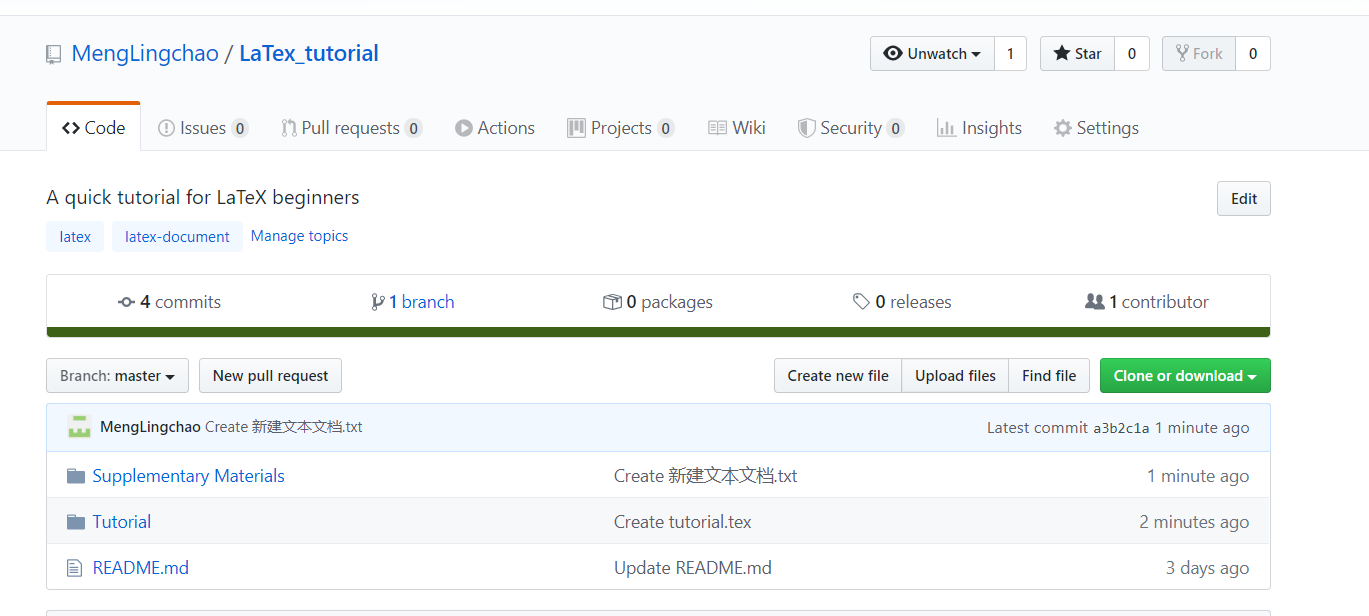
\includegraphics[width=0.7\linewidth]{figs/GitHub}
		\caption{GitHub Repository}
		\label{fig:github}
	\end{figure}
	
\end{frame}

\begin{frame}{Outline}
	\tableofcontents
\end{frame}

\section{Introduction}
\begin{frame}
	\sectionpage
\end{frame}

\begin{frame}[fragile]{What's \LaTeX?}
\LaTeX\ (pronounced either “Lay-tech” or “Lah-tech”) 
	\begin{itemize}
		\item is based on Tex, a typesetting system designed by Donald Knuth in 1978 for high quality digital typesetting.
		\item is a \textit{typesetting system} and \textit{programming language}, not a \textit{word processor}.
	\end{itemize}

\vskip 0.25cm
\begin{LTXexample}[caption={the typesetting nature of \LaTeX}]
This is \textbf{my} \emph{first} document prepared in \LaTeX. I \underline{typed} it on \today.
\end{LTXexample} 
\end{frame}

\begin{frame}{Why \LaTeX?}
\begin{itemize}
	\item Donald Knuth says that his aim in creating TEX is to beautifully
	typeset \textit{technical documents} especially those \textit{containing a lot of Mathematics}.
	\item Most English journals have their own \LaTeX\ template.
	\item Even for ordinary text, \LaTeX\ is also a good choice.
\end{itemize}
\end{frame}

\begin{frame}{Installation}
	On Windows, users have two main choices of TeX system to install: \alert{TeX Live} or \alert{MiKTeX}. I highly recommend Tex Live for the following reasons
	\begin{itemize}
		\item The standard installer for MiKTeX installs 'just the basics' and uses on-the-fly installation for anything else you need; the standard install for TeX Live is 'everything' (about 4.5 Gb!).
		\item Real-time updates.
		\item Faster compilation (especially in case of graphics files)
	\end{itemize}
\end{frame}

\begin{frame}{Installation}
There are many different editors of \LaTeX.
\begin{itemize}
\item professional \LaTeX\ editors, such as TeXstudio, TeXwork.
\item edit \LaTeX files using Vim, Sublime Text, Visual Code, etc.
\end{itemize}
 \vskip 0.75cm

Recommend Tex Live with TexStudio, you can refer to https://blog.csdn.net/zywhehe/article/details/83113214. 
\end{frame}

\begin{frame}{Installation}
 \begin{figure}
 	\centering
 	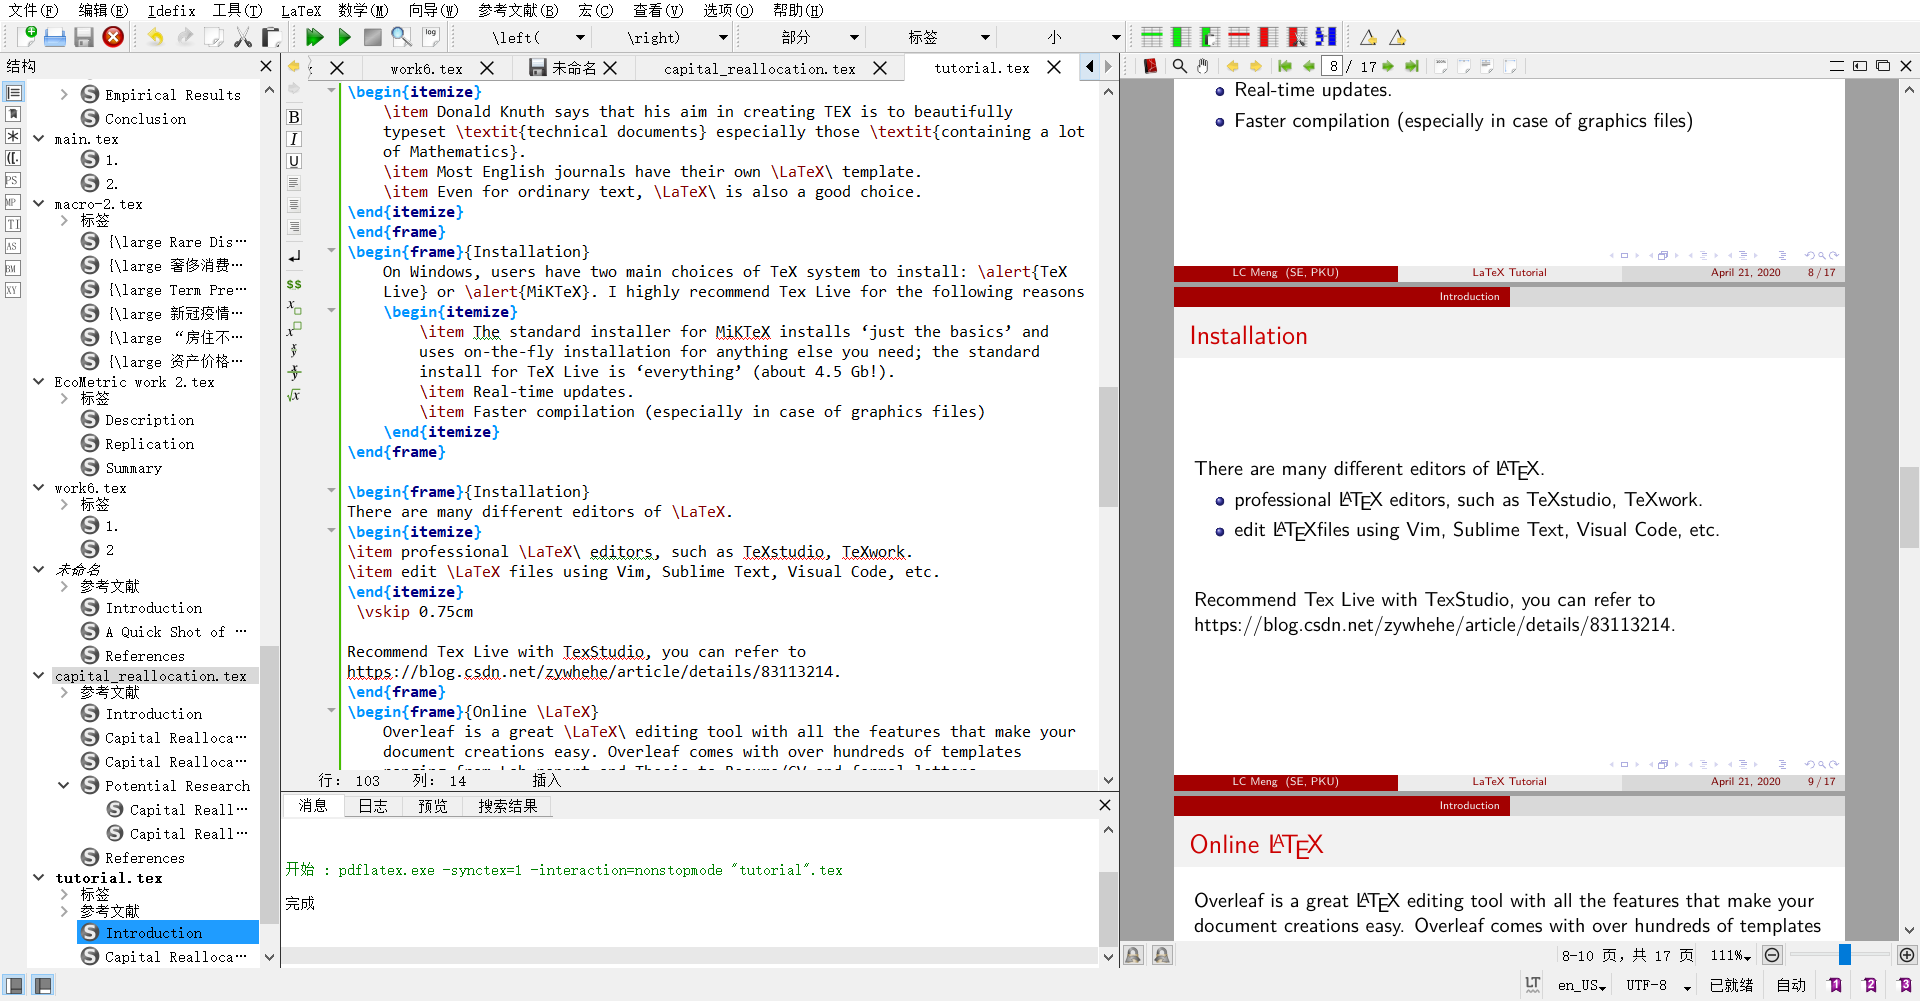
\includegraphics[width=0.85\linewidth]{figs/TeXstudio}
 	\caption{TeXstudio}
 	\label{fig:texstudio}
 \end{figure}
 
\end{frame}
\begin{frame}{Online \LaTeX}
	
	Overleaf(https://www.overleaf.com/) is a great \LaTeX\ editing tool with all the features that make your document creations easy. Overleaf comes with over hundreds of templates ranging from Lab report and Thesis to Resume/CV and formal letters. 
\begin{figure}
	\centering
	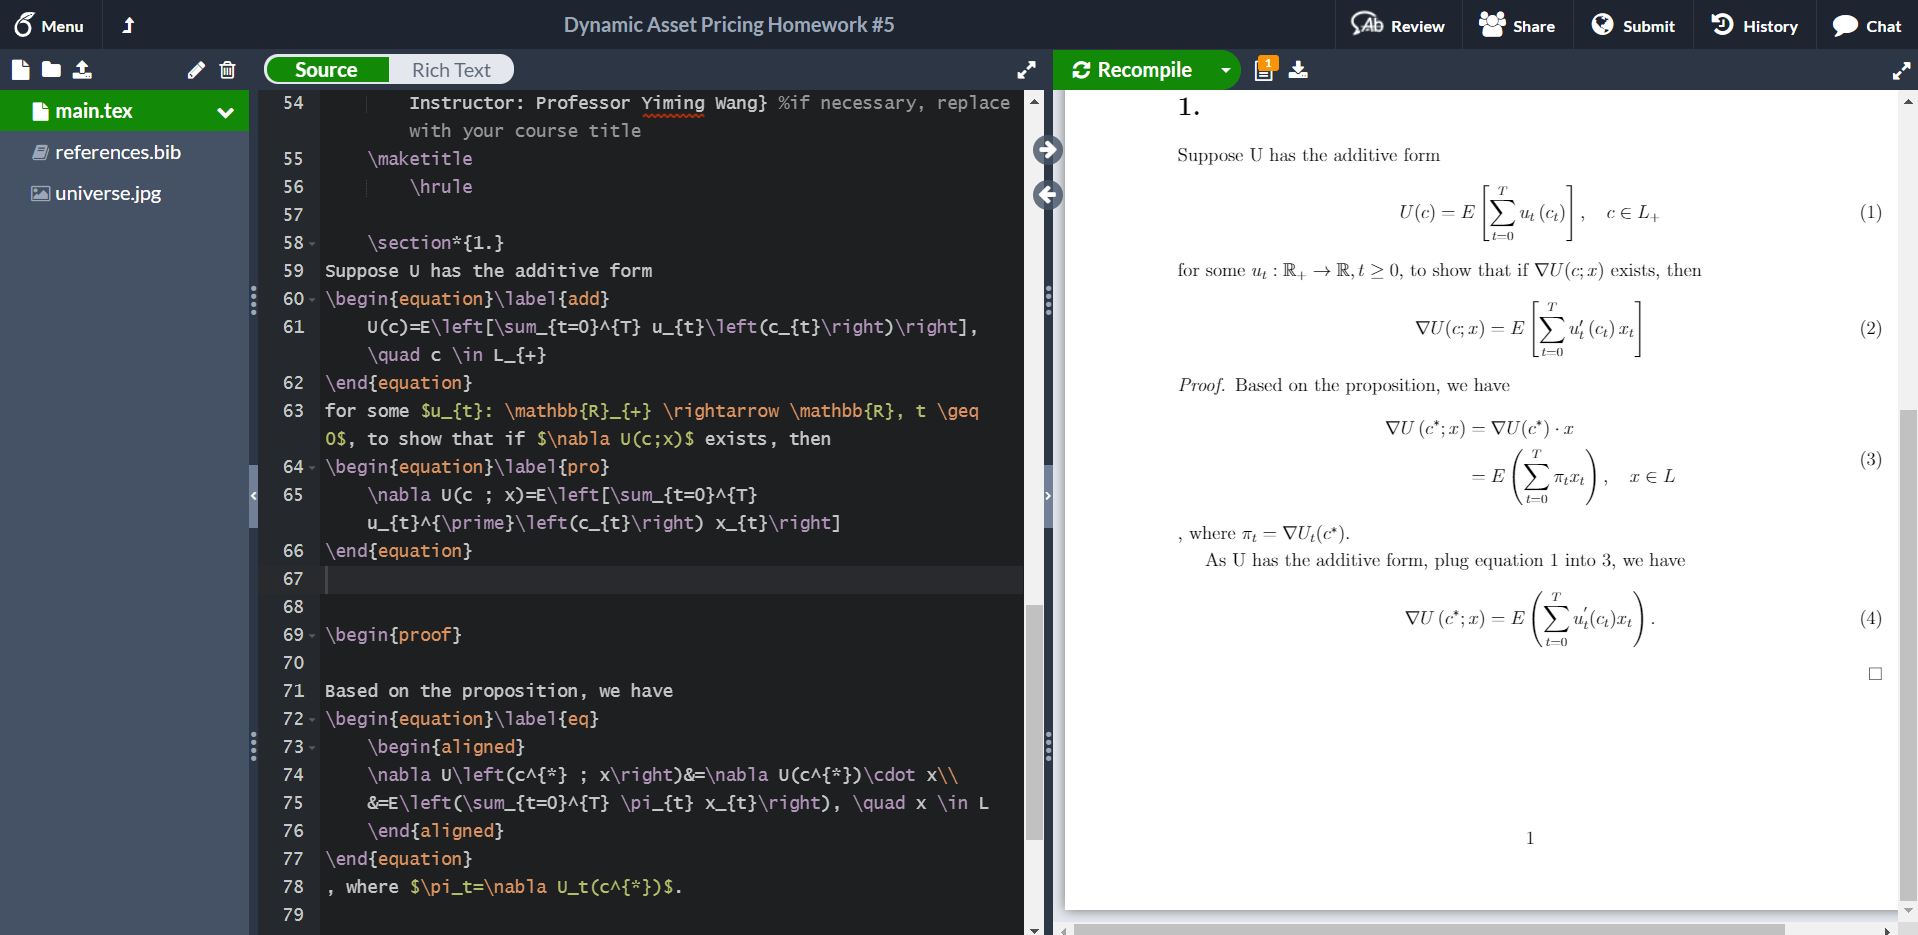
\includegraphics[width=0.7\linewidth]{figs/overleaf}
	\caption{Overleaf website}
	\label{fig:overleaf}
\end{figure}
\end{frame}


\section{\LaTeX\ Basic}


\begin{frame}
	\sectionpage
\end{frame}


\begin{frame}[fragile]{The basic structure of a \LaTeX\ file}
	\begin{enumerate}
		\item The \textit{documentclass} command: define the property of the file
		\begin{itemize}
			\item article, beamer, report, thesis, letter, book
		\end{itemize}
		\item Preamble: including the packages, format the article.
		\item Begin and end of the document: the main body of the file.
	\end{enumerate}
\vskip 0.5cm
	\begin{lstlisting}
	\documentclass[options]{article}
	Preamble (for LATEX commands only)
	\begin{document}
	Document text (text with embedded LATEX commands)
	\end{document}
	\end{lstlisting}
\end{frame}

\begin{frame}{title}
	内容...
\end{frame}

\begin{frame}[fragile]
	\begin{LTXexample}[caption={the basic document structure}]
	\documentclass[a4paper,12pt]{article}
	\title{My First Document}
	\author{My Name}
	\date{\today}
	\maketitle
	\begin{document}
		A sentence of text.
	\end{document}

\end{LTXexample}
\end{frame}

\begin{frame}[fragile]{Basic Typesetting}
	\begin{itemize}
		\item Simply enter your content in most times, just like using word or txt.
		\cprotect\item When you need to start a new paragraph, add \verb+\par+ in the end or empty one line between two paragraphs.
	\end{itemize}

\vskip 0.5cm
\begin{LTXexample}[caption={new paragraph}]
The first paragraph.\par
The second paragraph.

The third paragraph.
\end{LTXexample}
\end{frame}

\section{Basic Typesetting}

\begin{frame}
	\sectionpage
\end{frame}
\begin{frame}[fragile]{Font effects}
There are \LaTeX\ commands for a variety of font effects:
\begin{LTXexample}[caption={Font effects}]
\textbf{hello world}

\textit{hello wolld}

\underline{hello world}

\textsc{hello world}

\textrm{hello world}
\end{LTXexample}
\end{frame}

 \begin{frame}[fragile]{Colored text}
	\begin{itemize}
		\cprotect\item Include the xcolor package in the preamble by \verb+\usepackage{xcolor}+.
		\cprotect\item Also can define customized color \verb+\definecolor{myred}{RGB}{231, 76, 60}+.
	\end{itemize}
	 
	 \begin{LTXexample}[caption={Colored text}]
\begin{itemize}
	\item \textcolor{red}{Red}
	\item \textcolor{gray}{Gray}
	\item \textcolor{myred}{Myred}
\end{itemize}
	 \end{LTXexample}
\end{frame}



\section{Capital Reallocation: the Theory}
\begin{frame}
	\sectionpage
\end{frame}

\section{Potential Research}
\begin{frame}
	\sectionpage
\end{frame}

\subsection{Capital Reallocation in China Market}
\begin{frame}
	\begin{centering}
		{\small \begin{beamercolorbox}[center]{part title}
			\usebeamerfont{section title}\insertsubsection\par
		\end{beamercolorbox}}
	\end{centering}
\end{frame}

\subsection{Capital Reallocation and Empirical Asset Pricing}
\begin{frame}
	\begin{centering}
		{\small \begin{beamercolorbox}[center]{part title}
				\usebeamerfont{section title}\insertsubsection\par
		\end{beamercolorbox}}
	\end{centering}
\end{frame}

\section{References}
\begin{frame}
	\sectionpage
\end{frame}


\bibliographystyle{jf}
\bibliography{ref}
\end{CJK*}
\end{document}
